%        File: homework.tex
%     Created: 日 5月 20 09:00 下午 2018 C
% Last Change: 日 5月 20 09:00 下午 2018 C
%
\documentclass[UTF8,noindent]{ctexart}
\usepackage[a4paper,left=2.0cm,right=2.0cm,top=2.0cm,bottom=2.0cm]{geometry}
\usepackage{hyperref}
\usepackage{url}
\usepackage{graphicx}
\usepackage{amsmath}
\usepackage{amssymb}
\usepackage{enumitem}
\usepackage{tikz}
\usepackage{float}
\usepackage{listings}
\usepackage{xcolor}
\lstset{language = c,numbers=left, keywordstyle= \color{ blue!70 },commentstyle=\color{red!50!green!50!blue!50}, frame=shadowbox, rulesepcolor= \color{ red!20!green!20!blue!20 } 
} 
\usetikzlibrary{graphs}
\title{$Chapter\ 5-HW03$}
\author{$2015K8009929049$\ 冯吕}
\date{\today}
\begin{document}
\maketitle
\zihao{5}
\CJKfamily{zhsong}
\section*{$Homework\ 3$}

$5.4.4$解:
\begin{itemize}
  \item $(1)$
  \begin{center}
	\begin{tabular}{l l }
	  $S\rightarrow if (C) S_1\ else\ S_2$ & $L_1=new()$\\
	  & $L_2=new()$\\
	  & $C.true = L_1$\\
	& $C.false = L_2$\\
	& $S1.next = S.next$\\
	& $S2.next = S.next$\\
	& $S.code = C.code \parallel lable \parallel L_1\parallel S_1.code$\\
	& $\parallel goto\ S.next\parallel lable \parallel L_2\parallel S2.code$
	\end{tabular}
  \end{center}

\item $(2)$
  \begin{center}
	\begin{tabular}{l l }
	  $S\rightarrow do\  S_1\ while(C)$ & $L_1=new()$\\
	  & $L_2=new()$\\
	  & $C.true = L_1$\\
	  & $C.false = S.next$\\
	& $S1.next = L_2$\\
	%& $S2.next = S.next$\\
	& $S.code = label\parallel L_1 \parallel S_1.code$\\
	& $\parallel lable \parallel L_2\parallel C.code$
	\end{tabular}
  \end{center}
\item $(3)$
  \begin{center}
	\begin{tabular}{ll}
	  $S\rightarrow '\{'L'\}'$ & $L.next = S.next$\\
	  & $S.code = L.code$\\
	  $L\rightarrow L_1 S$ & $M= new()$\\
	  &   $L_1.next = M$\\
	  & $S.next = L.next$\\
	  & $L.code = L_1.code \parallel label \parallel M\parallel S_1.code$\\
	  $L\rightarrow \epsilon$ & $L.code = ""$
	\end{tabular}
  \end{center}
\end{itemize}

$5.5.4$解:
$(1)$
\begin{figure}[H]
  \centering
  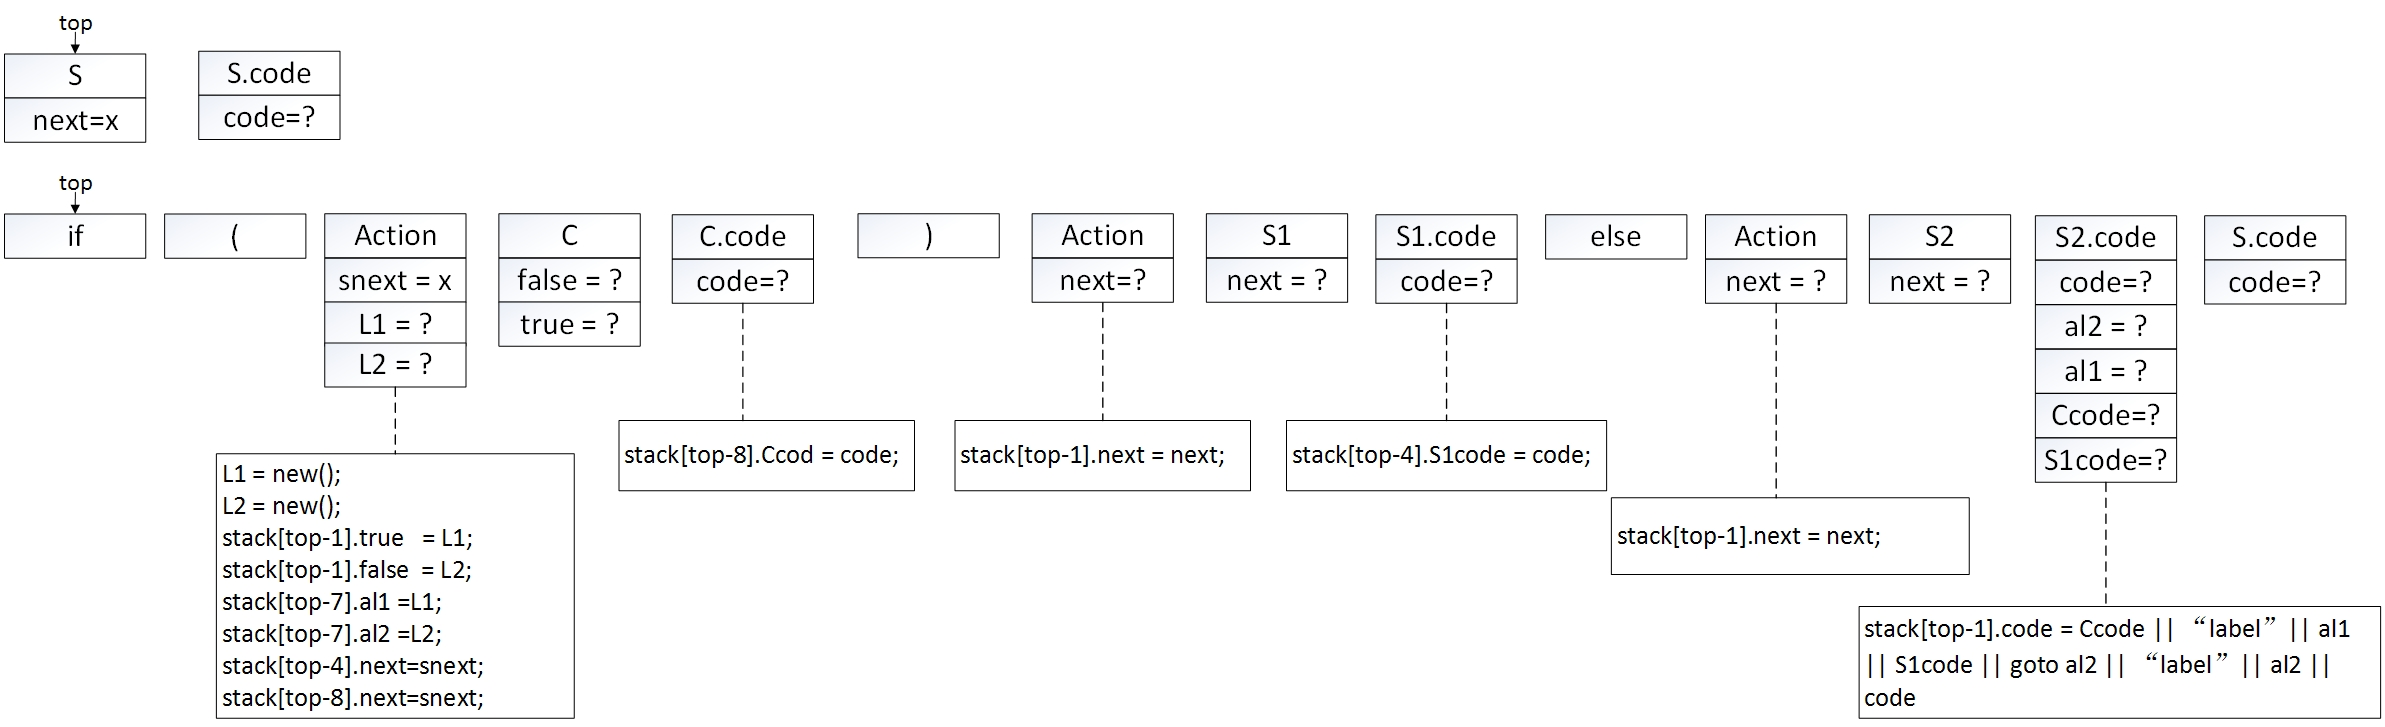
\includegraphics[scale = 0.3]{./fig/5-5-4-a.jpg}
\end{figure}

$(2)$
\begin{figure}[H]
  \centering
  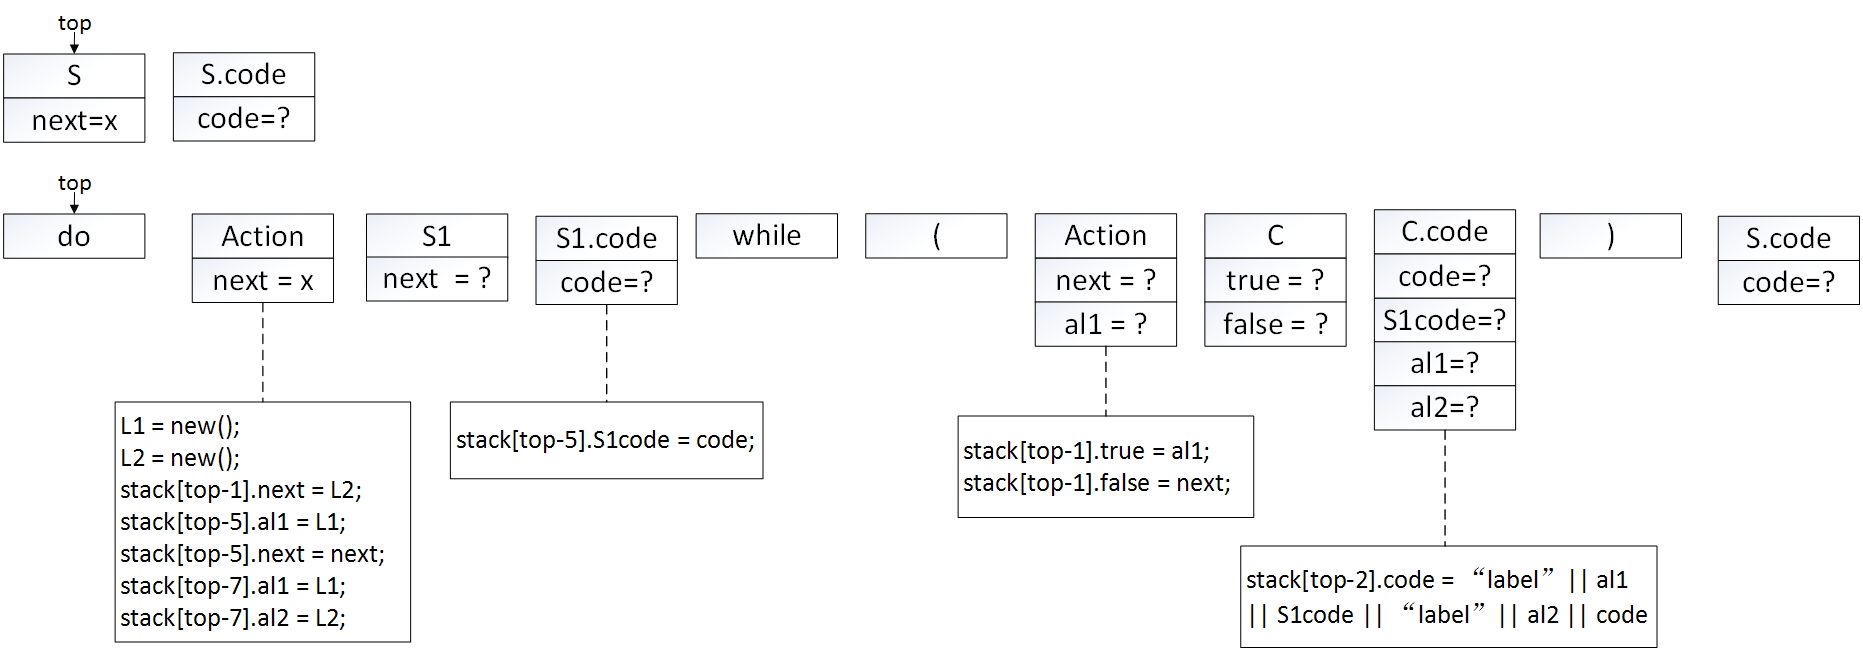
\includegraphics[scale = 0.3]{./fig/5-5-4-b.jpg}
\end{figure}

$(3)$
对文法消除左递归:
\begin{align*}
  &S\rightarrow '\{'L'\}'\\
  & L\rightarrow L'\\
  & L'\rightarrow SL'\mid \epsilon
\end{align*}
\begin{figure}[H]
  \centering
  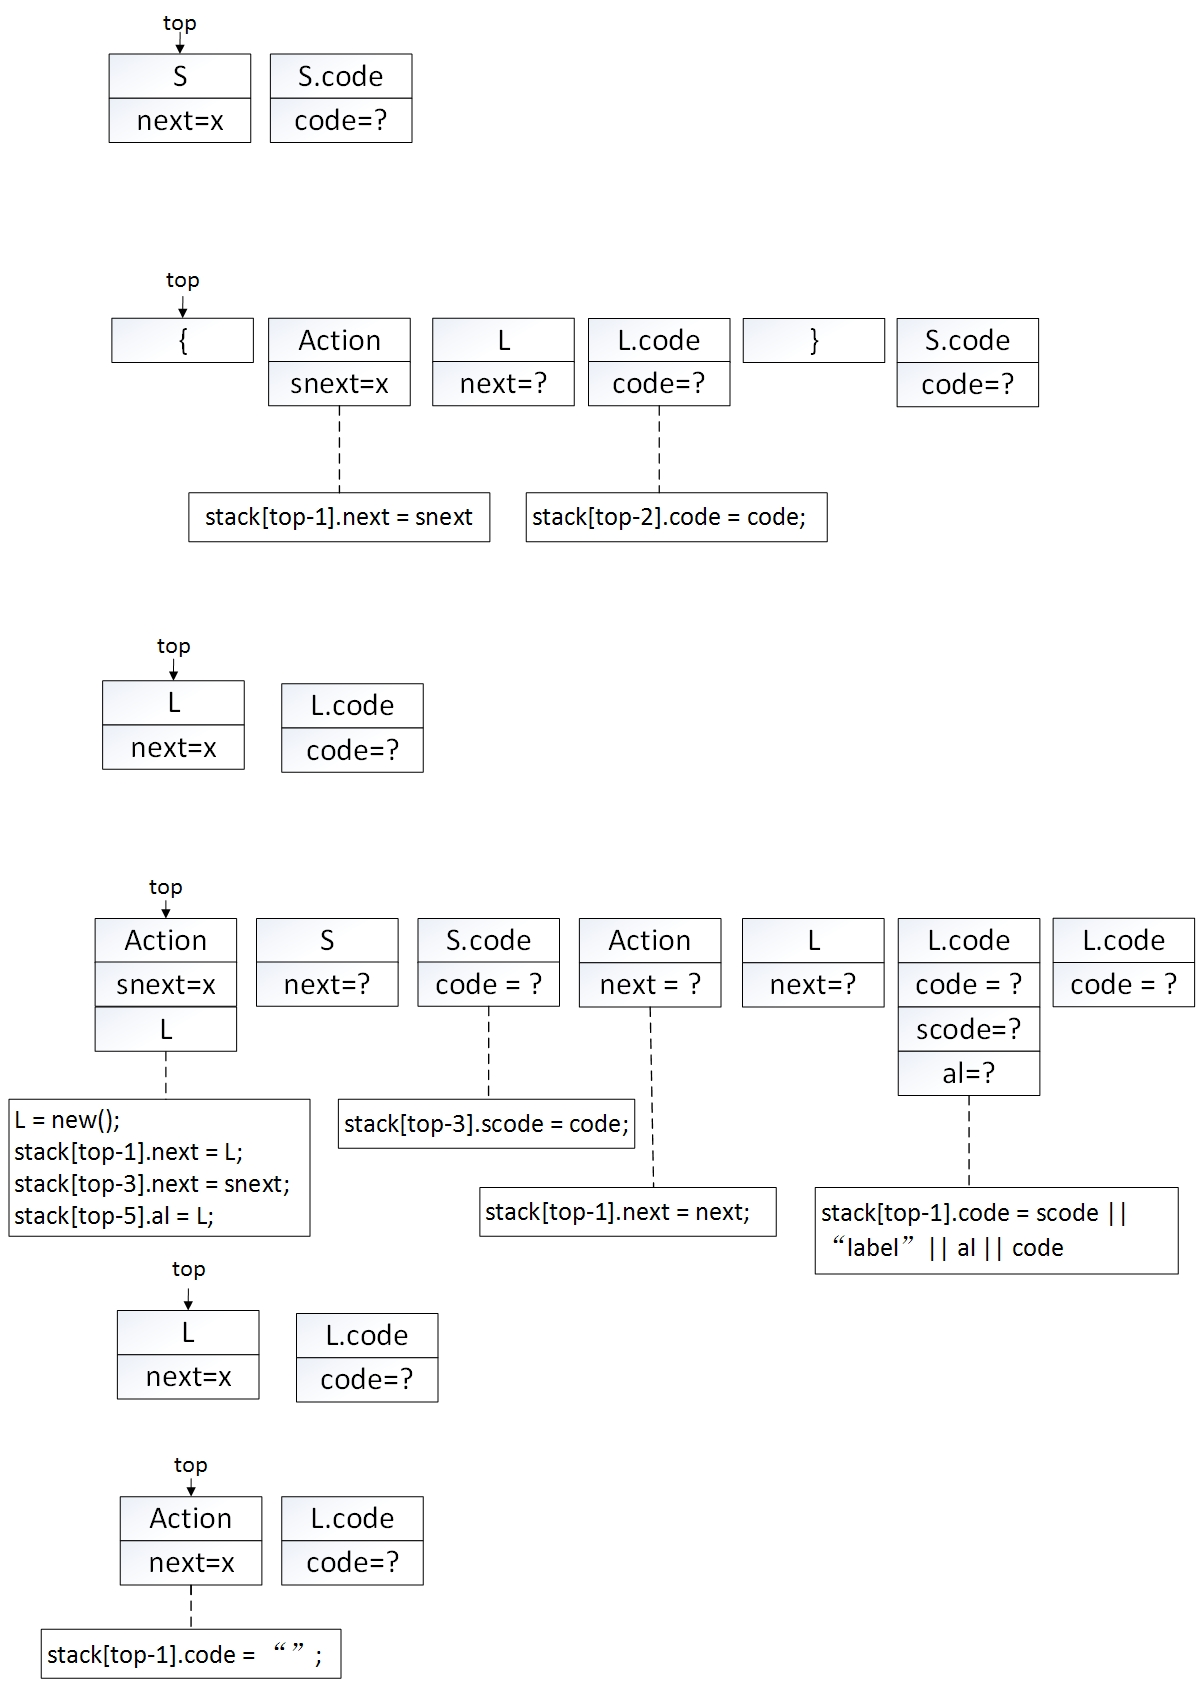
\includegraphics[scale = 0.4]{./fig/5-5-4-c.jpg}
\end{figure}

$5.5.5$解:
$(1)$
\begin{figure}[H]
  \centering
  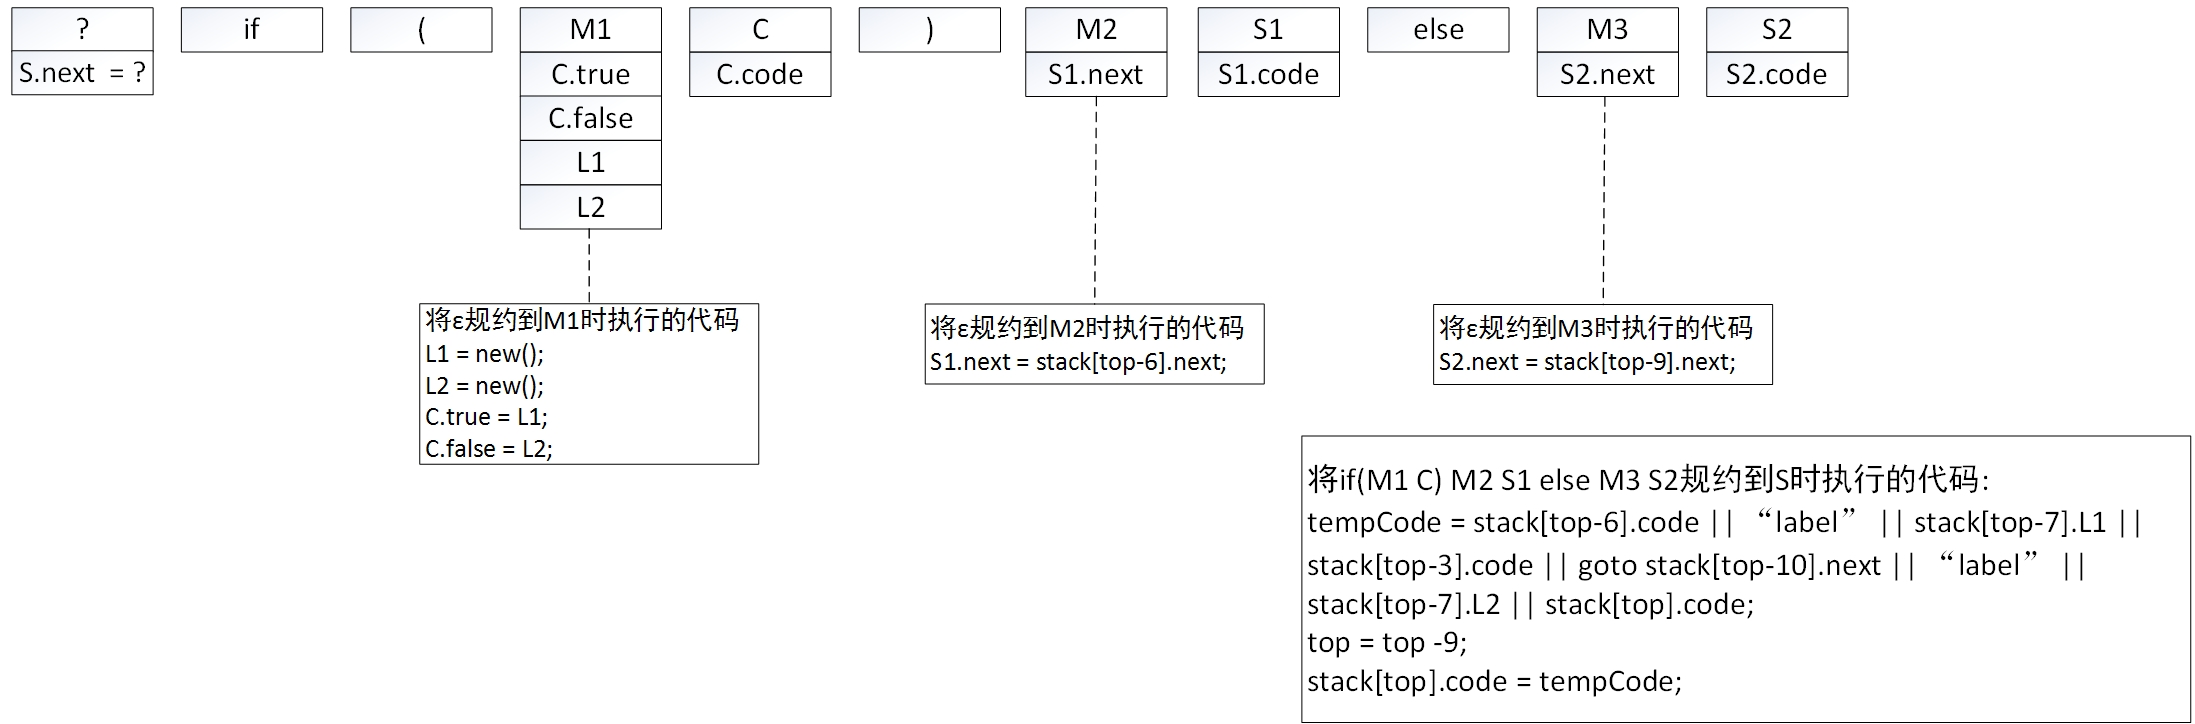
\includegraphics[scale = 0.3]{./fig/5-5-5-a.jpg}
\end{figure}

$(2)$
\begin{figure}[H]
  \centering
  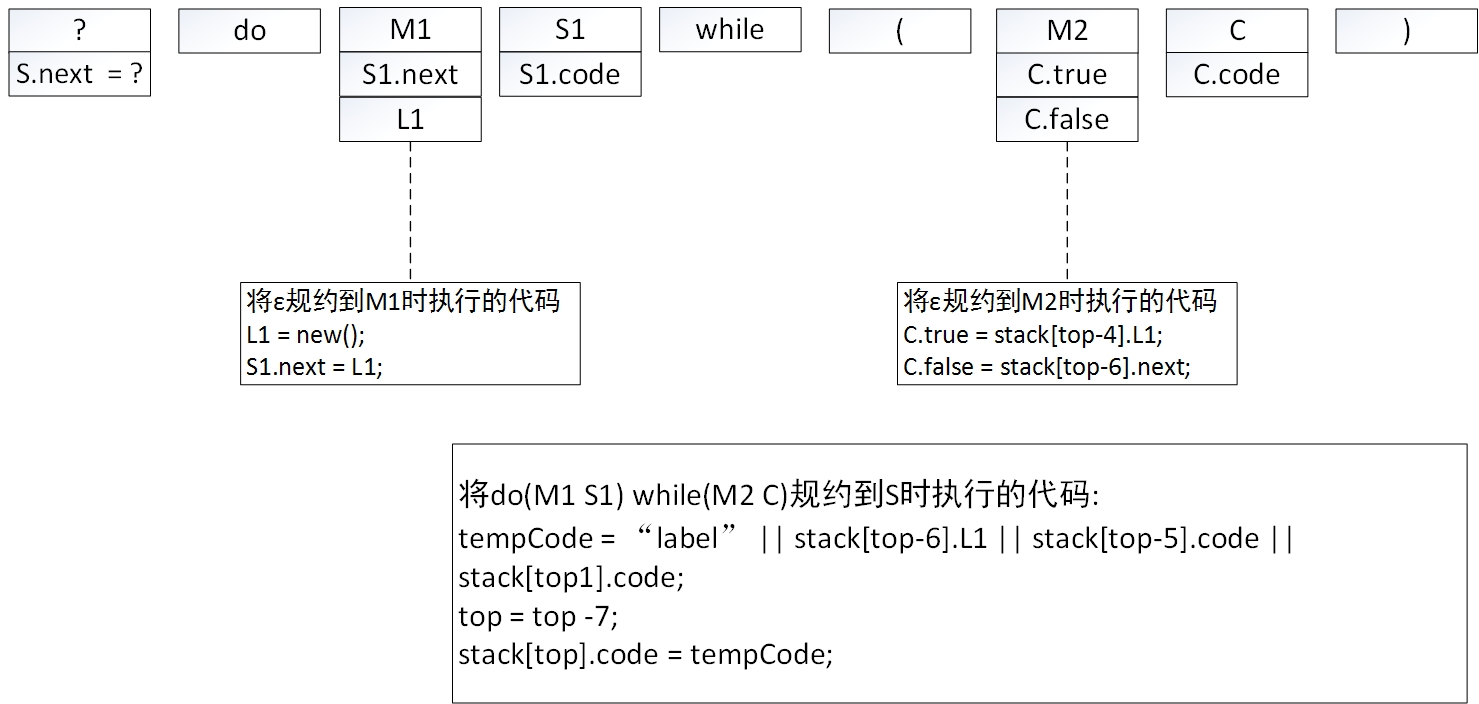
\includegraphics[scale = 0.3]{./fig/5-5-5-b.jpg}
\end{figure}

$(3)$
对文法消除左递归:
\begin{align*}
  &S\rightarrow '\{'L'\}'\\
  & L\rightarrow L'\\
  & L'\rightarrow SL'\mid \epsilon
\end{align*}
\begin{figure}[H]
  \centering
  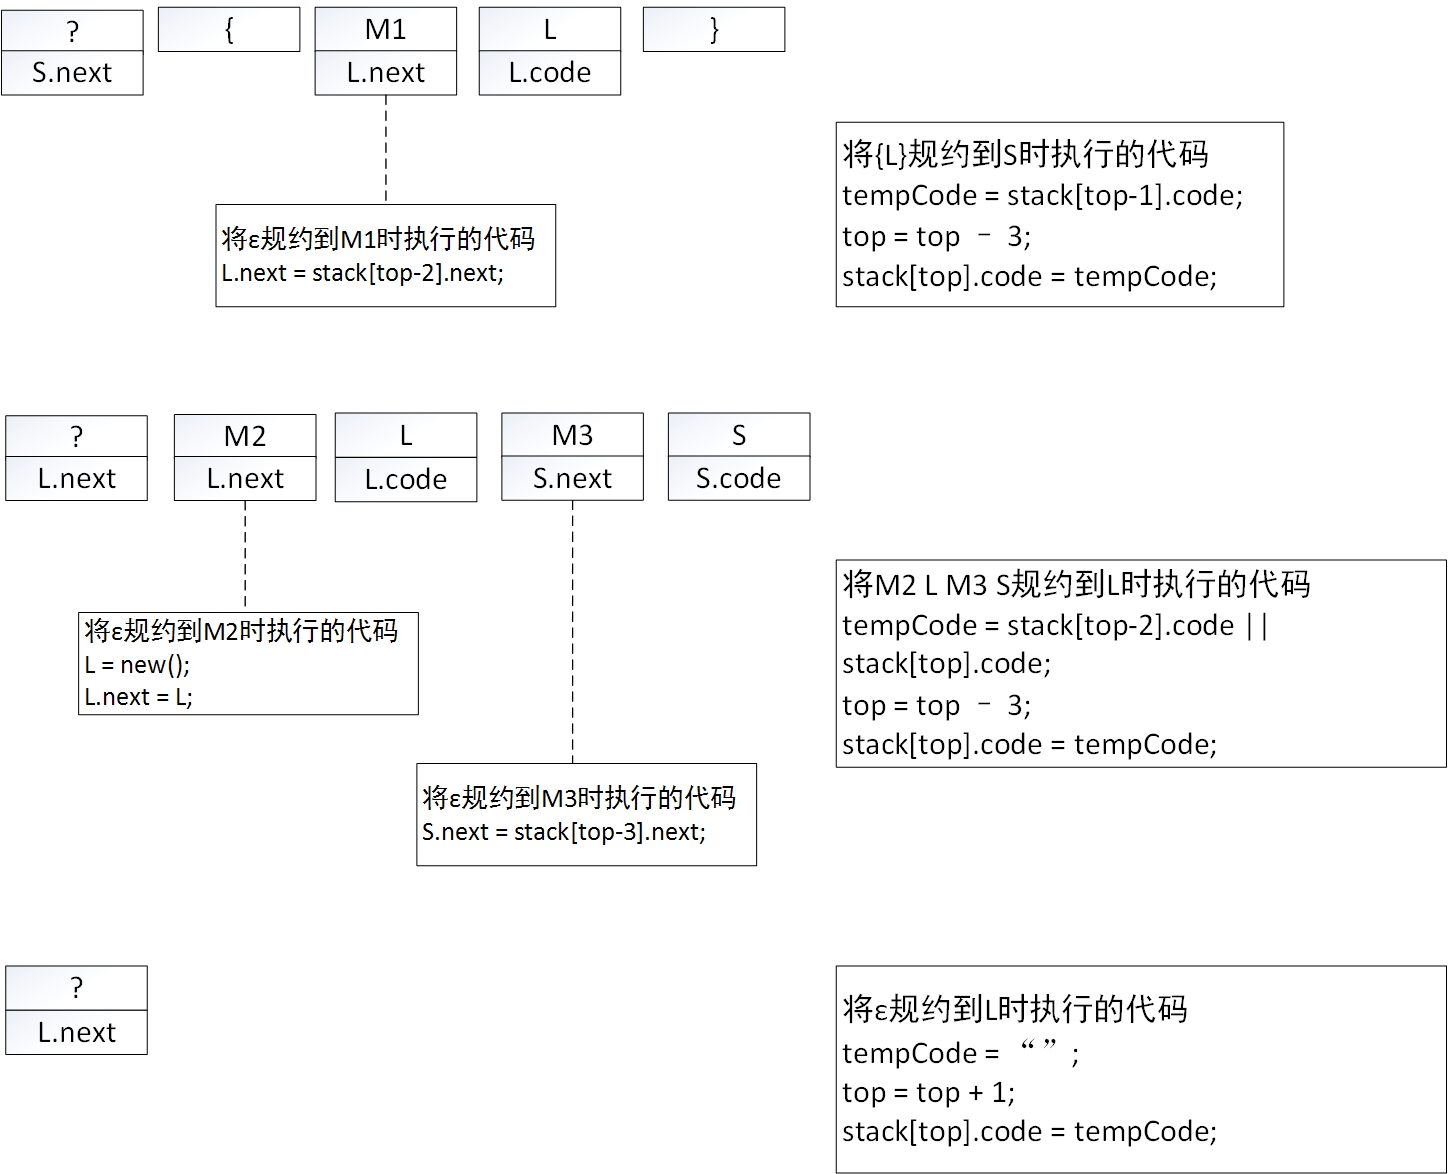
\includegraphics[scale = 0.4]{./fig/5-5-5-c.jpg}
\end{figure}
\end{document}
